\chapter{Bestaande situatie}

\todo[inline]{Herbekijk (zie ook comments)}

\section{SNMP Data Retriever}
\label{snmp-data-retriever}
De SNMP Data Retriever is het stuk software dat NetworkMining zelf ontwikkeld heeft voor de bevraging van netwerkcomponenten via SNMP.
Alhoewel het de bedoeling is om netwerkcomponenten te ondervragen over bijvoorbeeld hun routetabel of \gls{arptabel},
is het geen probleem om ook alle andere soorten toestellen te ondervragen, bijvoorbeeld werkstations van werknemers of
telefoontoestellen die verbonden zijn met het netwerk. De retriever laat je toe om een lijst van op te vragen toestellen op te geven.
Om te weten welke gegevens moeten opgevraagd worden bij elk toestel, moet aan elk toestel een toesteltype toegewezen worden.
De toesteltypes maak je zelf aan en bevatten een lijst van de op te vragen gegevens voor dat type.
Hieronder geven we een overzicht van de verschillende configuratiemogelijkheden die de \nwmretriever{} aanbiedt.

We bespreken ook de databankstructuur die door de \nwmretriever{} gebruikt wordt om de resultaten in weg te schrijven
en geven ook een globaal overzicht van hoe de software te werk gaat.

\todo[inline]{Relevant om dit hier nog eens te herhalen? V}
Bij de aanvang van de masterproef was het zo dat de retriever reeds ingezet werd voor kleine en middelgrote netwerken.
De bedoeling van de masterproef is om de nodige aanpassingen te doen zodat de retriever ook vlot kan ingezet worden voor grote netwerken,
van 1000 toestellen en meer.
% Het plan is om eind dit jaar de software ook te kunnen gebruiken voor het netwerk van Telenet. \todo{Mag Telenet vermeld worden?}

\todo[inline]{Samenvatting van de werking van de retriever? GET- \& GETNEXT-requests, wegschrijven van de resultaten in een DB}

\todo[inline,caption=bestaande-snmp-retriever]{Uitleg over bestaande SNMP Data Retriever. \\
Vandaag in gebruik bij NetworkMining voor kleine netwerken.
Bedoeling om te kunnen inzetten op grote netwerken zoals dat van Telenet. \\
Beschrijving huidige functionaliteit, hoe werkt de software, configuratie zie hieronder.}

\subsection{Configuratie}
\label{snmp-data-retriever-configuratie}
Er zijn drie manieren waarop de retriever kan geconfigureerd worden. De belangrijkste,
en wellicht de enige waar de eindgebruiker mee in aanraking zal komen is het XML-configuratiebestand.
Een aantal opties kunnen ook doorgeven worden aan de hand van argumenten bij het oproepen van het programma.
De laatste manier is via nog een configuratiebestand: het \emph{AppConfig}-bestand. De laatste twee mogelijkheden
zullen hoogstwaarschijnlijk eenmalig geconfigureerd worden bij de installatie van de software en verder nooit meer gewijzigd worden.

% We bespreken de configuratiemogelijkheden die aangeboden worden door elke optie en hoe die ingesteld moeten worden.

\todo[inline]{3 manieren om de retriever te configureren, zie de puntjes hieronder.}

\subsubsection{XML-configuratiebestand}
Zoals gezegd is dit de belangrijkste manier om de retriever te configureren.
De twee belangrijkste dingen die je kunt configureren zijn wat voor types toestellen er zijn en de lijst van IP-adressen van die toestellen.
Een voorbeeld van een definitie van een toesteltype zie je in \cref{xmlconfig-typedefinition}.
Het toesteltype heet \emph{General} en als er een toestel van dat type bevraagd wordt,
moet er een SNMP walk gedaan worden van de \textit{system} boomtak met als \gls{oid} 1.3.6.1.2.1.1.
Dit is dezelfde boomtak die we eerder hebben gezien in \cref{boomstructuur}.
De system boomtak is verplicht aanwezig op alle SNMP-toestellen, vandaar de naam van het toesteltype.
Het \gls{mib}-bestand waarin die tak gedefiniëerd is heet \emph{RFC1213-MIB}.
Deze gegevens vind je terug als de attributen van de SNMP walk-opdracht in het configuratiebestand.
Een toesteltype moet niet beperkt zijn tot een enkele SNMP walk. Ze kan ook bestaan uit meerdere SNMP walk-opdrachten,
of zelfs een SNMP GET-opdracht voor een enkele \gls{oid}.

% Make a float of the code listing so it doesn't get broken up in a page break.
\begin{lstlisting}[language=XML, float=h, caption={Definitie van een toesteltype in het XML-configuratiebestand}, label=xmlconfig-typedefinition]
<deviceType name="General">
	<snmpWalk oid="1.3.6.1.2.1.1" mib="RFC1213-MIB" name="system" />
</deviceType>
\end{lstlisting}

Nadat de toesteltypes gedefiniëerd zijn kun je de IP-adressen opgeven van alle toestellen die opgevraagd moeten worden.
Bij de opsomming van de toestellen hoort natuurlijk ook hun toesteltype die we eerder gedefiniëerd hebben.
In \cref{xmlconfig-devicedefinition} zie je dat de definitie van een toestel bestaat uit drie attributen: een arbitrair gekozen naam, zijn IP-adres of hostnaam en zijn toesteltype. 

\begin{lstlisting}[language=XML, float=h, caption={Definitie van een toestel in het XML-configuratiebestand}, label=xmlconfig-devicedefinition]
<device name="atlas2a1.intec.ugent.be" ip="atlas2a1.intec.ugent.be" type="Bridge" />
\end{lstlisting}

De overige opties zijn die voor een databaseconnectiestring, de communitystring, de locatie van de \gls{mib}-bestanden en de SNMP-timeout waarde.
Dit is hoelang gewacht wordt (in milliseconden) op een response na het versturen van een SNMP-request.

\begin{lstlisting}[language=XML, float=h, caption={Overige opties in het XML-configuratiebestand}, label=xmlconfig-misc]
<database value="Database=snmpdb;Data Source=localhost;User Id=networkminer;Password=SomePassword;Port=3306;old syntax=yes" />
<snmpCommunity get="public" />
<MIBpath value=".\MIBs" />
<snmpTimeout value="3000" />
\end{lstlisting}


\subsubsection{Argumenten}
Bij het oproepen van de retriever kun je optioneel enkele argumenten meegeven.
De belangrijkste twee zijn \emph{inputfile} en \emph{clearresults}.
Met het eerste argument geef je de locatie mee van het XML-configuratiebestand.
Clearresults zorgt ervoor dat resultaten van een vorige retrieval gewist worden, zodat je met een schone lei begint.
In \cref{retriever-argumenten} zie je een voorbeeld van hoe je deze argumenten moet gebruiken.

\begin{lstlisting}[float=h, caption={Oproepen van SNMP Data Retriever met twee argumenten}, label=retriever-argumenten]
SNMPDataRetrieval.exe "-clearresults" "-inputfile=config\snmp.xml"
\end{lstlisting}


\todo[inline, caption={Argumenten van retriever}]{
Zie ParseCommandLineAttributes():

\begin{itemize}
	\item clearresults
	
	\item noretrieve
	
	\item getdevicesfromquery
	
	\item serial
	
	\item inputfile
\end{itemize}
}

\subsubsection{AppConfig}
Met het AppConfig-bestand zal de eindgebruiker normaal niet mee in contact komen.
Ze bevat de mogelijkheid om het loglevel te veranderen zodat meer of minder logging informatie wordt weggeschreven in het logbestand.
De databaseconfiguratiestring kan hier ook opgegeven worden,
maar indien er in het XML-configuratiebestand ook een databank opgegeven wordt, dan wordt de laatste gebruikt.
Na het vervangen van het loggingframework (zie \cref{profiling}) komen er enkele loggingopties bij in dit bestand.
Zo kun je naast het loglevel ook extra uitvoermogelijkheden opgeven: naar een tekstbestand, naar het consolescherm, naar een databank of een combinatie.
Ook het logformaat kan hier desgewenst aangepast worden.

\subsection{Databankstructuur}
\label{snmp-data-retriever-db}
Tijdens het uitvoeren van de \nwmretriever{} worden er een drietal tabellen aangemaakt: \textit{types}, \textit{devices} en \textit{results}.
In de eerste tabel worden de toesteltypes opgeslagen.
Een voorbeeld zie je in \cref{fig-db-types}.
Daar werden twee toesteltypes gedefinieerd: bridge en router.
Voor elk toesteltype zijn er een aantal opdrachten (GET- of walkopdrachten), samen met hun datatype, \gls{oid}, \gls{mib}-bestand en naam.

\begin{figure}[h]
	\centering
	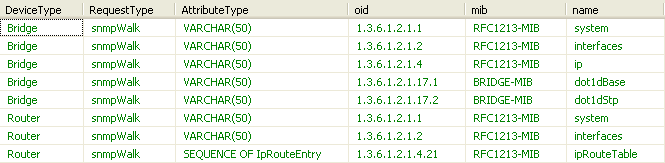
\includegraphics[scale=0.50]{figures/database/types}
	\caption{Tabel van toesteltypes en hun opdrachten}
	\label{fig-db-types}
\end{figure}

De toestellen zelf worden opgeslagen in de devices tabel.
In \cref{fig-db-devices} zie je een toestel met zijn IP-adres of hostnaam, het toesteltype en zijn communitystring.

\begin{figure}[h]
	\centering
	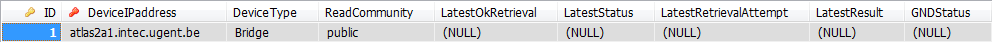
\includegraphics[scale=0.40]{figures/database/devices}
	\caption{Tabel van toestellen}
	\label{fig-db-devices}
\end{figure}

De laatste tabel bevat de opgehaalde gegevens.
Een aantal resultaten zie je in \cref{fig-db-results}.
Elk resultaat bevat de host, de \gls{oid}, het attribuutnaam (dat wordt samengesteld uit de naam van de \gls{mib} en de naam van de \gls{oid}),
de waarde van het resultaat en de datum waarop ze werd opgehaald.

\begin{figure}[h]
	\centering
	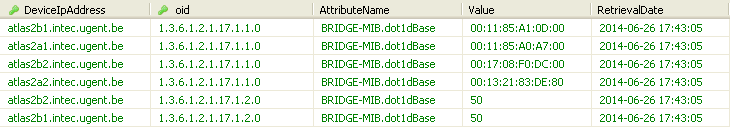
\includegraphics[scale=0.50]{figures/database/results}
	\caption{Tabel van resultaten}
	\label{fig-db-results}
\end{figure}


\subsection{Werking}
\label{werking}

In deze paragraaf geven we een \textit{high-level} overzicht van de werking van de \nwmretriever{}.
Bij het analyseren van de applicatie met een profiler wordt hier ook naar verwezen om te weten wat elke methode juist doet.

De \nwmretriever{} begint eerst en vooral met de \textit{Initialize}-methode op te roepen,
die verantwoordelijk is voor de configuratie en het opzetten van de databankverbinding.
Zowel de commandlineparameters als het XML-configuratiebestand worden hier verwerkt.
Na het inlezen van de configuratie wordt de databankverbinding opgezet met de gegevens uit de configuratie.

Nadat de basisconfiguratie werd ingelezen door de Initialize-methode worden de toesteltypes (devicetypes) ingelezen uit het XML-configuratiebestand.
Indien nodig wordt er in de databank een nieuwe devicetypestabel aangemaakt en worden de toesteltypes daarin opgeslagen.
Hetzelfde gebeurt voor de te bevragen toestellen.
Ten slotte wordt er ook, indien nodig de results tabel aangemaakt om de opgehaalde gegevens in weg te schrijven.

Daarna kan het ophalen van de gegevens beginnen.
De lijst van de te bevragen toestellen wordt overlopen, en om meerdere toestellen tegelijkertijd op te vragen
wordt voor elk toestel wordt een nieuwe thread gestart.
Het ophalen zelf gebeurt in de \textit{RetrieveFromDevice}-methode en elke thread voert die methode uit voor een toestel.

Er worden maximaal 50 threads aangemaakt dus er kunnen maar 50 toestellen tegelijkertijd opgevraagd worden.
Eens er 50 threads aangemaakt zijn wordt er gewacht tot een vorige thread klaar is om een nieuwe te starten.
De threads worden in een lijst bijgehouden en in een oude versie van de \nwmretriever{} werd na het starten van de eerste 50 threads gewacht op
de eerste thread om nieuwe threads aan te maken.

De RetrieveFromDevice-methode overloopt de lijst van instructies die moeten afgehandeld worden voor een bepaald toestel(type).
Dat kunnen ofwel enkelvoudige gegevens zijn die opgehaald moeten worden met een GET-request ofwel moet een SNMP walk gedaan worden van een bepaalde \gls{oid}.
Vervolgens worden de request(s) gestuurd naar dat toestel.
Nadat het antwoord is ontvangen worden alle variabelen die in dat antwoord zitten overlopen.
Er wordt gecontroleerd of de ontvangen gegevens relevant zijn (als ze onder de originele \gls{oid} vallen bij een SNMP walk),
en zoja wordt het gegeven weggeschreven in de databank met de \textit{InsertResultRow}-methode.
De InsertResultRow-methode doet niks meer dan het uivoeren van een SQL insert-query.
Gegevens worden dus een per een weggeschreven in de databank.
